\thispagestyle{endchapter}

\begin{tcolorbox}
\vspace{80pt}

\lettrine{T}{he} 18 year odyssey in the Hollow Mountain (\passage{Tolminski Migovec}) reached a notable milestone with the connection of \passage{Vrtnarija} to \passage{System Migovec}, making it the longest cave in Slovenia.

To put into words how much this means to the people who have spent years (even decades!) dedicating their free time to this exploration project is difficult. But Clewin (first expedition 1997) put it beautifully: "Everybody has a made a contribution, from surveying hundreds of meters of horizontal passages to pushing ridiculously tight rifts or squalid muddy dead ends to feeding hungry cavers in the bivvy."

Despite the success of the 2012 expedition, it is clear that there
remains a large amount of cave to be discovered in \passage{Vrtnarija} and
Migovec. In \passage{Vrtnarija}, the obvious areas to focus our attention
on include: the descent of the wet pitches at the end of \passage{Brezno
Slapov} and \passage{Invictus}, pushing the rift at the end of \passage{Milky
Way}, further exploration of \passage{Xanadu} and \passage{Lower Pleasures},
various unpushed leads in \passage{Watership Down} at the bottom, and a
second bolt climb to a window at \passage{Queen's Bedchamber} that seems to
be the continuation of the horizontal development found in \passage{Milky Way}.
Furthermore, as we now have the necessary know-how and equipment to bolt
climb, there are various `deep' leads to revisit from the 2003
expedition such as \passage{Strap on the Nitro}.

In some ways, we have the fortunate problem of almost being too
successful in recent years, as the leads are now fairly spread out and
getting further from camp each year. This year, it was common for
pushing trips to \passage{Watership Down} and
\passage{Invictus}/\passage{Atlantis} to take upwards of 21 hours.
Nonetheless, Camp \passage{X-Ray} remains the most likely camp due to its
central location and easy access to water -- however, an additional
lightweight 2 man camp nearer to the more remote locations is a strong
possibility.

Thanks to the connection there are also old leads in the old \passage{SysMig} that
are worth revisiting, especially around the \passage{Waterloo} area.

\name{Jarvist Moore Frost}



\end{tcolorbox}
	\backgroundsetup{	scale=1.1,
        color=black,
        opacity=1,
        angle=0,
        contents={%
                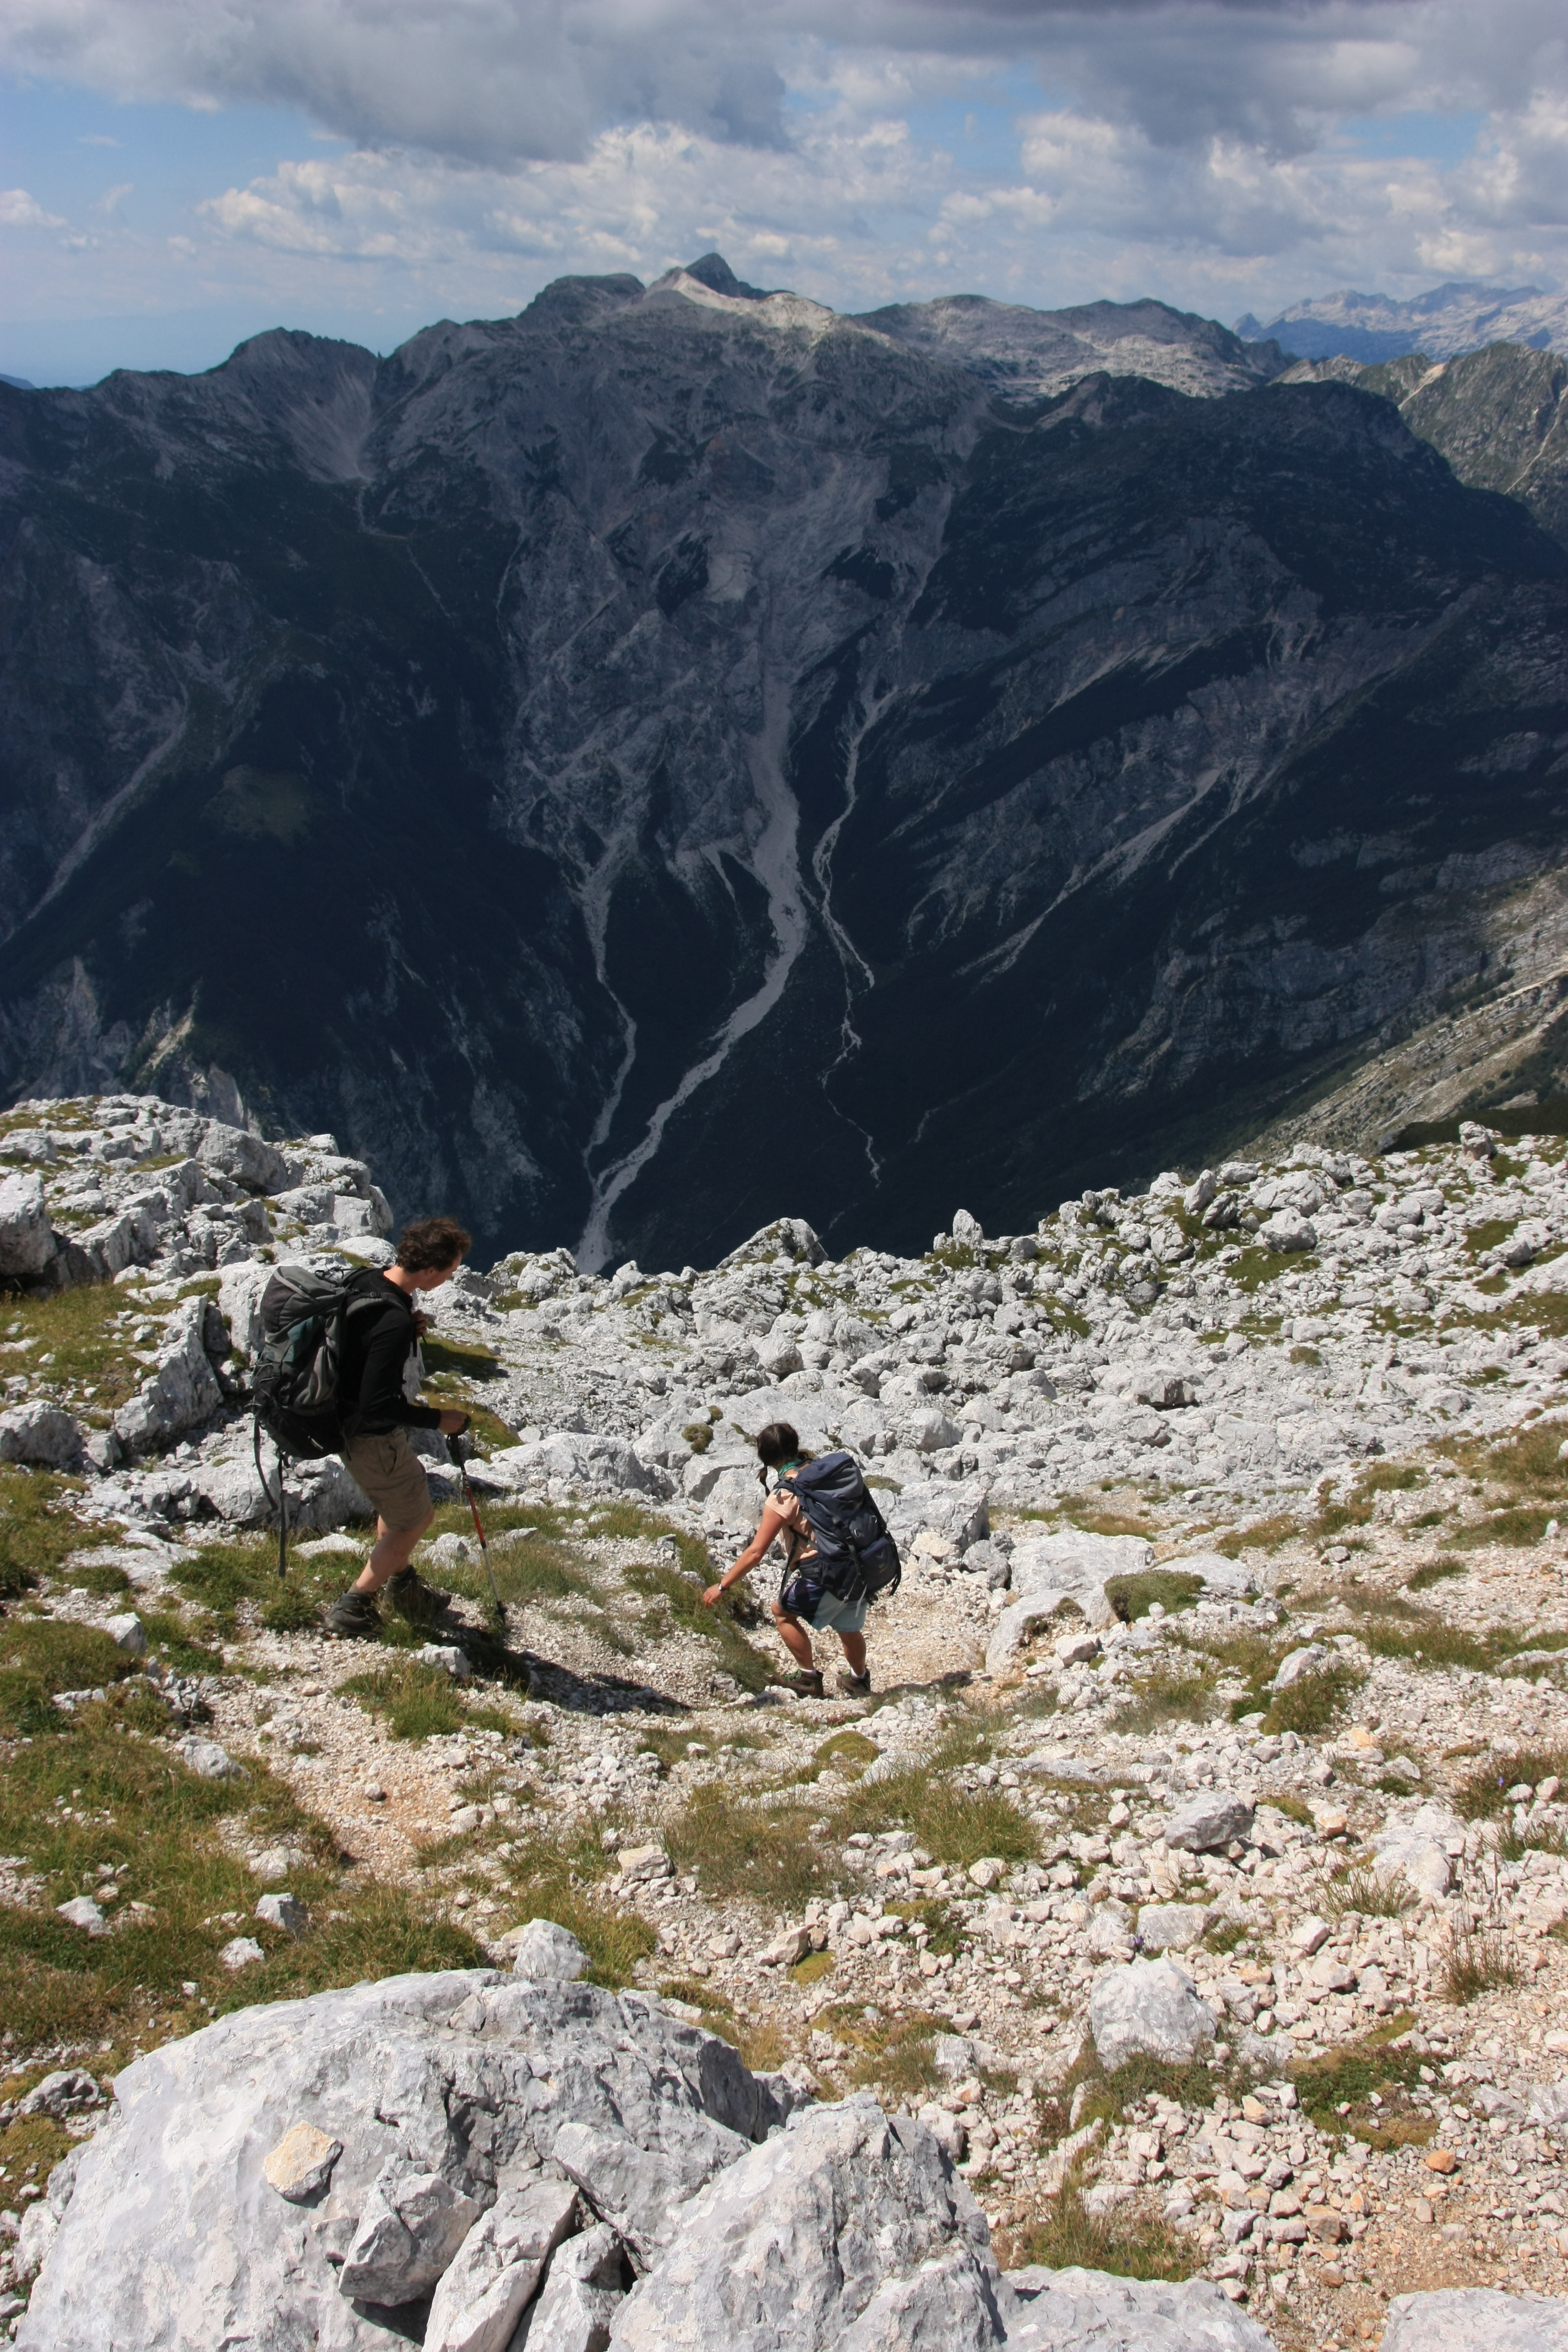
\includegraphics[height=\paperheight]{2012/outro/2012-08-10-0440-GergelyAmbrus-IMG_2249--orig.jpg}
        }
	}
\BgThispage